\section{Installation}

\begin{frame}{Systeminstallation och virtualenv}
  \begin{columns}
    \begin{column}{0.7\linewidth}
      Tre korta råd
      \begin{enumerate}
        \item Undvik installation i systemets Python
        \item Använd virtuella miljöer \emph{virtual env}
        \item Ha system för flera Python versioner installerade samtidigt
      \end{enumerate}

      Tänk på att
      \begin{itemize}
        \item Kan inte se vad som installerats direkt och vad som är beroenden på dessa
        \item Kan inte på ett generellt sätt låsa beroenden i flera led
      \end{itemize}
    \end{column}
    \begin{column}{0.3\linewidth}
      \begin{figure}
        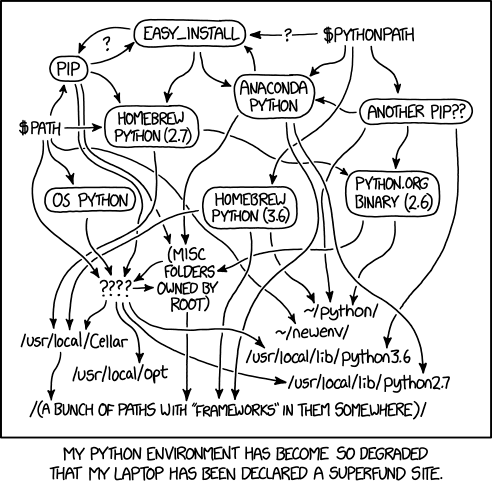
\includegraphics[width=\linewidth,keepaspectratio]{fig/python_environment}
        \caption{Randall Munroe, xkcd nr 1987}
      \end{figure}
    \end{column}
  \end{columns}
\end{frame}

\begin{frame}{Virtualenv - hantera moduler}
  \begin{itemize}
    \item Lokala paket per miljö/projekt
    \item Lätt "avinstallation" genom att ta bort mappen
    \item Skapa i skalet eller via IDE och aktiveras med aktiveringsskript\\
          \mintinline{shell-session}{python3 -m venv venv}\\
  \end{itemize}

  Glöm inte ignorera mappen i git!
\end{frame}

\begin{frame}{pyenv - hantera versioner}
  \begin{itemize}
    \item Olika Python-version per projekt
    \item Installera versioner oberoende av systemets pakethanterare
    \item Automatisk aktivering i specifika mappar med \texttt{.python-version} filer
    \item Installera med plugins för virtualenv-stöd
  \end{itemize}

  \vfill

  \begin{figure}
    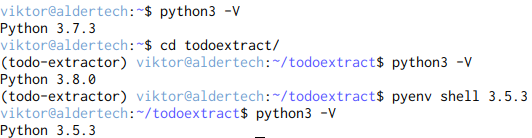
\includegraphics[width=0.8\linewidth,keepaspectratio]{fig/pyenv}
  \end{figure}
\end{frame}

\begin{frame}{pipx - hantera "binärer"}
  \begin{itemize}
    \item Isolerar Python program i separata venv
    \item Kan både installera och köra direkt
    \item Enkel uppdatering av allt installerat \mintinline{shell-session}{pipx upgrade-all}
    \item \emph{Kan ha flera versioner av samma program, men måste då manuellt symlänka}
  \end{itemize}

  Installera med \mintinline{shell-session}{pip3 install pipx}

  Bör vara \emph{den enda} paketet som är installerat i systemets Python
\end{frame}
